% \begin{figure}
%     \centering
%     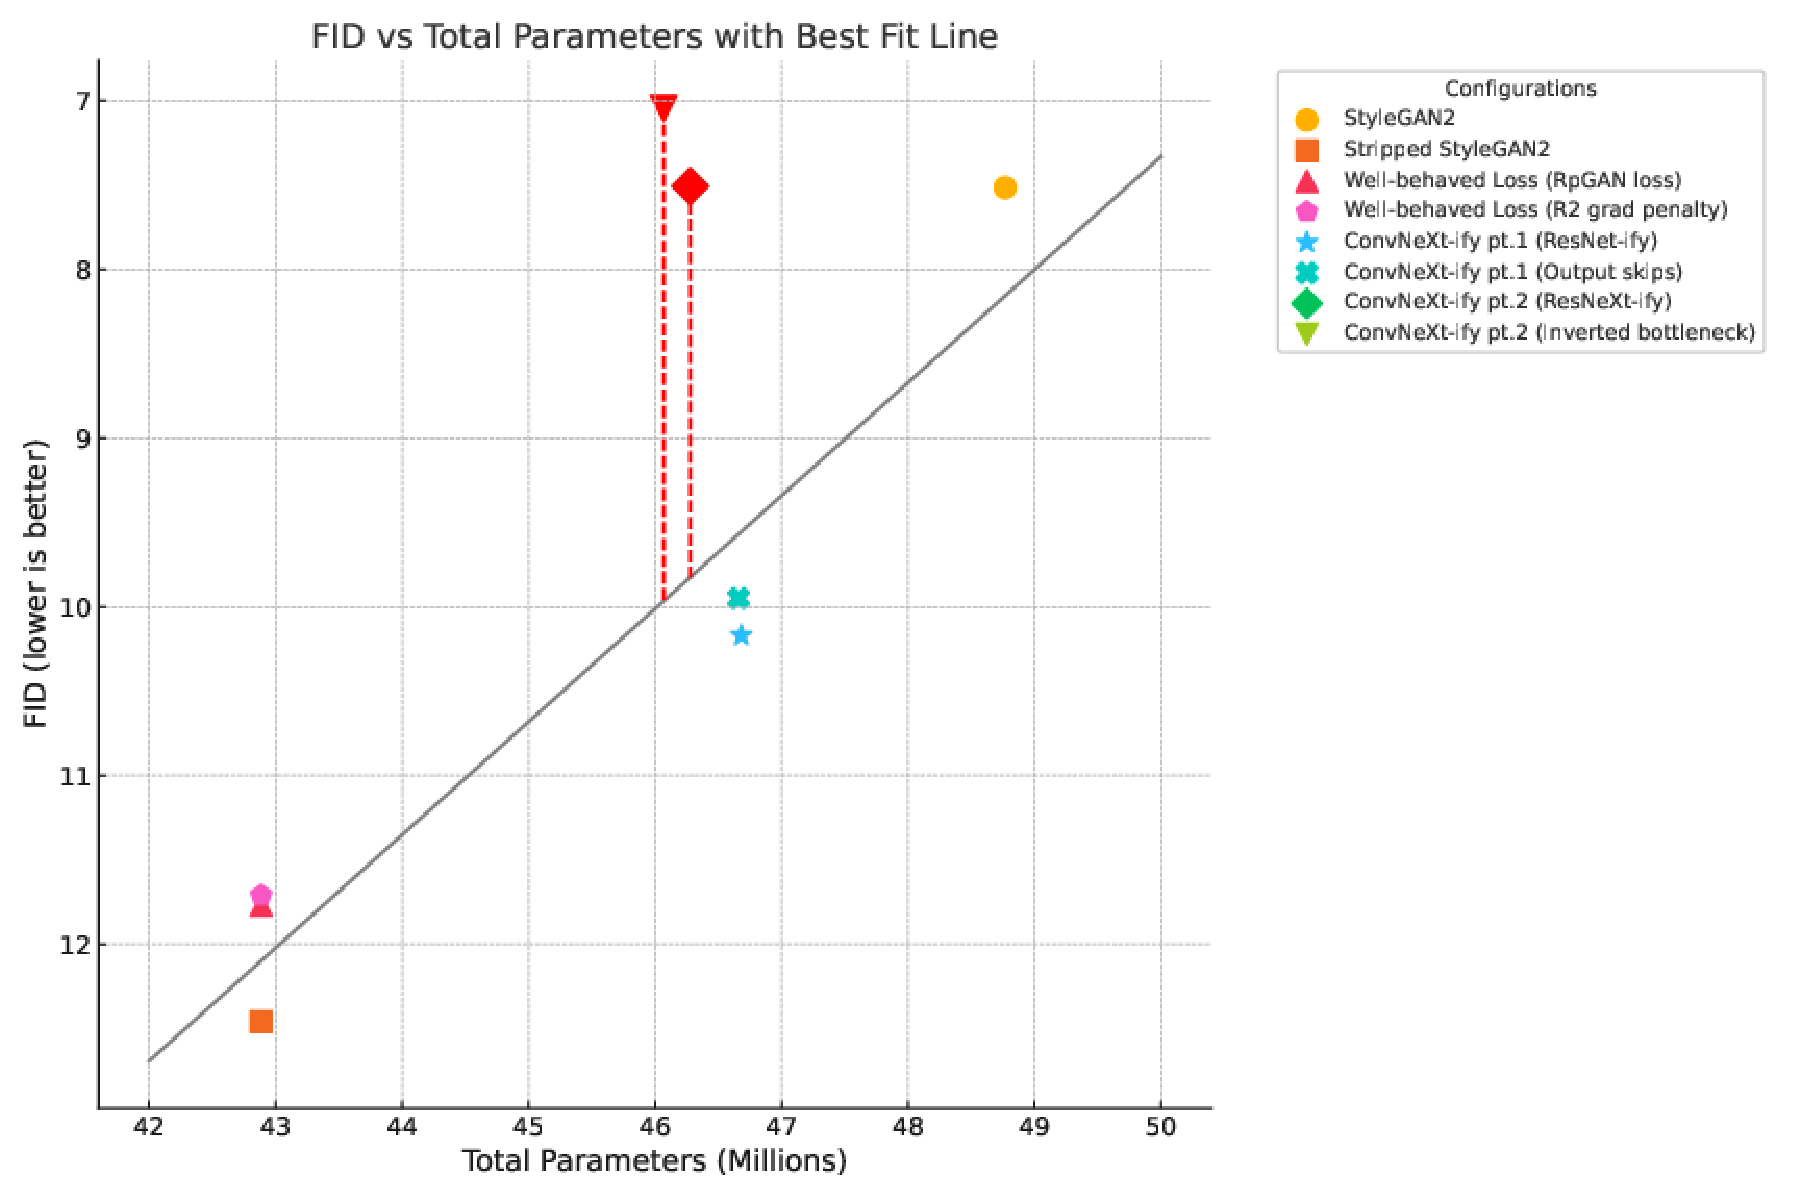
\includegraphics{figures/FID-vs-Params-Plot.eps}
%     \caption{This scatter-plot shows the FID performance of our model on FFHQ-256 vs the number of parameters when only trained for 5million steps}
%     \label{fig:fid-vs-params-ablation}
% \end{figure}


\section{A Roadmap to a New Baseline --- \modelName}
\label{sec:roadmap}

% \vk{What about naming the new GAN that is being proposed? SimpleGAN...?}\jt{R3GAN...?}

% \vk{My main comment about this section is that it reads like mix of methods and experiments: all the experimental details/results (e.g., we set the learning rate to $10^{-4}$) should be under experiments (but you can still describe the key important takeaways here, e.g., we need a smaller learning rate)}

The well-behaved RpGAN + $R_1$ + $R_2$ loss alleviates GAN optimization problems, and lets us proceed to build a minimalist baseline---\modelName---with recent network backbone advances in mind~\cite{convnext,metaformer}. Rather than simply state the new approach, we will draw out a roadmap from the StyleGAN2 baseline~\cite{sg2ada}. This model (Config A; identical to~\cite{sg2ada}) consists of a VGG-like~\cite{vgg} backbone for $G$, a ResNet $D$, a few techniques that facilitate style-based generation, and many tricks that serve as patches to the weak backbone. Then, we remove all non-essential features of StyleGAN2 (Config B), apply our loss function (Config C), and gradually modernize the network backbone (Config D-E).


We evaluate each configuration on FFHQ $256\times256$~\cite{sg1}. Network capacity is kept roughly the same for all configurations---both $G$ and $D$ have about 25\ M trainable parameters. Each configuration is trained until $D$ sees 5\ M real images. We inherit training hyperparameters (\eg, optimizer settings, batch size, EMA decay length) from Config A unless otherwise specified. We tune the training hyperparameters for our final model and show the converged result in Sec.~\ref{sec:exp}.

%\paragraph{StyleGAN2 (Config A).}This configuration is identical to the baseline~\cite{sg2ada} with the style-based generator and all tricks enabled.  

\vspace{-0.3cm}
\paragraph{Minimum baseline (Config B).}
\begin{wraptable}[21]{r}{8cm}
\vspace{-0.5cm}
\resizebox{1\linewidth}{!}{
\begin{tabular}{ l r c c c } 
\toprule
   & \multicolumn{1}{l}{Configuration}  & FID$\downarrow$                    & G \#params              & D \#params               \\ 
\midrule
A  & \multicolumn{1}{l}{StyleGAN2}  & 7.516                  & 24.767M                  & 24.001M                   \\
\midrule
B  & \multicolumn{1}{l}{Stripped StyleGAN2}                                                                                                                                                                                                                                                                                                                                                                                                                 &                        &                          &                           \\ 
   & \begin{tabular}[c]{@{}r@{}}\textcolor{red}{- $z$ normalization}\\ \textcolor{red}{- Minibatch stddev}\\ \textcolor{red}{- Equalized learning rate}\textcolor{red}{}\\\textcolor{red}{- Mapping network}\\ \textcolor{red}{- Style injection}\\ \textcolor{red}{- Weight mod / demod}\\ \textcolor{red}{- Noise injection}\\ \textcolor{red}{- Mixing regularization}\\ \textcolor{red}{- Path length regularization}\\ \textcolor{red}{- Lazy regularization}\textcolor{blue}{}\end{tabular} & \multirow{2}{*}{12.46} & \multirow{2}{*}{18.890M} & \multirow{2}{*}{23.996M}  \\ 
\midrule
C  & \multicolumn{1}{l}{Well-behaved Loss}                       &                        &                          &                           \\ 
 & \textcolor[rgb]{0,0.502,0.502}{+ RpGAN loss}                                                                                                                                                                                                                                                                                                                                                                                                                   & 11.77                                           & \multirow{2}{*}{18.890M} & \multirow{2}{*}{23.996M}                           \\ 
   & \textcolor[rgb]{0,0.502,0.502}{+ $R_2$ gradient penalty}                                                                                                                                                                                                                                                                                                                                                                                                & \multirow{1}{*}{11.65} &                          &                           \\ 
\midrule
D  & \multicolumn{1}{l}{ConvNeXt-ify pt.~1}                                                                                                                                                                                                                                                                                                                                                                                                                 &                        &                          &                           \\ 
 & \textcolor[rgb]{0,0.502,0.502}{+ ResNet-ify G $\&$ D}                                                                                                                                                                                                                                                                                                                                                                                                   & 10.17                  & 23.400M                  & \multirow{2}{*}{23.282M}  \\
   & \textcolor{red}{- Output skips}                                                                                                                                                                                                                                                                                                                                                                                                                         & 9.950 & 23.378M &                           \\ 
\midrule
E  & \multicolumn{1}{l}{ConvNeXt-ify pt.~2}                              &                        &                          &                           \\
 & \textcolor[rgb]{0,0.502,0.502}{+ ResNeXt-ify G $\&$ D}                                                                                                                                                                                                                                                                                                                                                                                                  & 7.507                  & 23.188M                  & 23.091M                   \\ 
   & \textcolor[rgb]{0,0.502,0.502}{+ Inverted bottleneck}                                                                                                                                         & 7.045 & 23.058M & 23.010M  \\ 
\bottomrule
\end{tabular}
}
\vspace{-0.25cm}
\caption{Effect of our simplification and modernization efforts evaluted on FFHQ-256.} 
\label{tab:roadmap}
\end{wraptable}

%To find the essential elements that contribute to StyleGAN2's success, 
We strip away all StyleGAN2 features, retaining only the raw network backbone and basic image generation capability. The features fall into three categories:
\begin{itemize}[leftmargin=10pt,itemsep=0pt,topsep=0pt]
\item Style-based generation: mapping network~\cite{sg1}, style injection~\cite{sg1}, weight modulation/demodulation~\cite{sg2}, noise injection~\cite{sg1}.
\end{itemize}\quad % JT: Weird but intential LaTeX
\begin{itemize}[leftmargin=10pt,itemsep=0pt,topsep=0pt]
\vspace{-0.25cm} % JT: Weird but intentional LaTeX
\item Image manipulation enhancements: mixing regularization~\cite{sg1}, path length regularization~\cite{sg2}.
\item Tricks: $z$ normalization~\cite{pggan}, minibatch stddev~\cite{pggan}, equalized learning rate~\cite{pggan}, lazy regularization~\cite{sg2}.
\end{itemize}

% Such features could be reintroduced as per application need (e.g., style injection). 
Following~\cite{sgxl,sg-t}, we reduce the dimension of $z$ to 64. The absence of equalized learning rate necessitates a lower learning rate, reduced from 2.5$\times$10\textsuperscript{-3} to 5$\times$10\textsuperscript{-5}. Despite a higher FID of 12.46 than Config-A, this simplified baseline produces reasonable sample quality and stable training. We compare this with DCGAN~\cite{dcgan}, an early attempt at image generation. Key differences include:
\begin{enumerate}[label=\alph*), noitemsep,topsep=0pt,leftmargin=24pt]
\item Convergent training objective with $R_1$ regularization.\label{item:convergent} 
\item Smaller learning rate, avoiding momentum optimizer (Adam $\beta_1=0$).\label{item:learning_rate} 
\item No normalization layer in $G$ or $D$.\label{item:normalization} 
\item Proper resampling via bilinear interpolation instead of strided (transposed) convolution.\label{item:resampling} 
\item Leaky ReLU in both $G$ and $D$, no tanh in the output layer of $G$.\label{item:activation} 
\item 4$\times$4 constant input for $G$, output skips for $G$, ResNet $D$.\label{item:input} 
\end{enumerate}

\textbf{Experimental findings from StyleGAN.} Violating \ref{item:convergent}, \ref{item:learning_rate}, or \ref{item:normalization} often leads to training failures.
%, contributing to the reputation that GANs as difficult to train. 
Gidel~\etal~\cite{ganmomentum} show that \emph{negative} momentum can improve GAN training dynamics. Since optimal negative momentum is another challenging hyperparameter, we do not use any momentum to avoid worsening GAN training dynamics. Studies suggest normalization layers harm generative models~\cite{sg2,edm2}. Batch normalization~\cite{bn} often cripples training due to dependencies across multiple samples, and is incompatible with $R_1$, $R_2$, or RpGAN that assume independent handling of each sample. Weaker data-independent normalizations~\cite{sg2,edm2} might help; we leave this for future work. Early GANs may succeed despite violating \ref{item:convergent} and \ref{item:normalization}, possibly constituting a full-rank solution~\cite{r1} to Eq.~\ref{eq:gan}.

Violations of \ref{item:resampling} or \ref{item:activation} do not significantly impair training stability but negatively affect sample quality. Improper transposed convolution can cause checkerboard artifacts, unresolved even with subpixel convolution~\cite{subpixel} or carefully tuned transposed convolution unless a low-pass filter is applied. Interpolation methods avoid this issue, varying from nearest neighbor~\cite{pggan} to Kaiser filters~\cite{sg3}. We use bilinear interpolation for simplicity. For activation functions, smooth approximations of (leaky) ReLU, such as Swish~\cite{swish}, GELU~\cite{gelu}, and SMU~\cite{smu}, worsen FID. PReLU~\cite{prelu} marginally improves FID but increases VRAM usage, so we use leaky ReLU.

All subsequent configurations adhere to \ref{item:convergent} through \ref{item:activation}. Violation of \ref{item:input} is acceptable as it pertains to the network backbone of StyleGAN2~\cite{sg2}, modernized in Config D and E.

% \paragraph{Minimum baseline (Config B).}
% To elucidate the implementation details that contribute to the success of StyleGAN2, we remove all the StyleGAN2 features until only the raw network backbone and basic image generation capability are retained. The list of removed features can be placed into three categories:
% \begin{itemize}
%     \item Style-based generation: mapping network~\cite{sg1}, style injection~\cite{sg1}, weight modulation / demodulation~\cite{sg2}, noise injection~\cite{sg1}.
%     \item Image manipulation enhancements: mixing regularization~\cite{sg1}, path length regularization~\cite{sg2}.
%     \item Tricks: $z$ normalization~\cite{pggan}, minibatch stddev~\cite{pggan}, equalized learning rate~\cite{pggan}, lazy regularization~\cite{sg2}.
% \end{itemize}
% The first two categories are technically orthogonal to our work; we remove them along with the tricks as our goal is to build a minimalist baseline and they can be reintroduced to our model in the future. \aaron{For this work, we want to keep our baseline as simple as possible, and demonstrate that many of these additions are not necessary for training a state of the art GAN. Instead, we ask what the simplest architecture one can design that can be used to train a GAN.}\vk{Do you include back the things you remove? Curious why / why not} Following~\cite{sgxl,sg-t}, we decrease the dimension of $z$ to 64. The removal of equalized learning rate necessitates a significantly lower learning rate and we decrease the learning rate from $2.5\times10^{-3}$ to $5\times10^{-5}$, any higher learning rate cripples training. This highly simplified baseline, despite achieving a considerably worse FID of 12.46, produces quite reasonable sample quality and training is stable. We compare this baseline against DCGAN~\cite{dcgan}, a barely working early GAN attempt at image generation. Notable differences include:
% \begin{enumerate}[label=\alph*)]
%     \item Convergent training objective with $R_1$ regularization.
%     \item Smaller learning rate, not using a momentum optimizer (Adam $\beta_1=0$).
%     \item Neither $G$ nor $D$ uses any normalization layer.
%     \item Proper resampling via bilinear interpolation instead of strided (transposed) convolution.
%     \item Leaky ReLU in both $G$ and $D$, no tanh in the output layer of $G$.
%     \item $4\times4$ constant input for $G$, output skips for $G$, ResNet $D$.
% \end{enumerate}

% \vk{Part B too verbose and many of these details can be in appendix  or removed }
% Our experiments show that any violation of a), b), or c) can easily lead to training failures, and these violations likely earned GANs the reputation of being hard to train. Gidel~\etal~\cite{ganmomentum} show that momentum not only should be avoided for GAN optimization, but \emph{negative} momentum might even improve GAN training dynamics. Since the optimal negative momentum is another hard to tune hyperparameter, we simply do not use any momentum to at least not worsen the GAN training dynamics. Recent studies~\cite{sg2,edm2} on GANs and diffusion models show that normalization layers harm generative models. Batch normalization~\cite{bn} in particular often cripples training as it establishes dependency across multiple samples and it is therefore incompatible with $R_1$, $R_2$ or RpGAN, all of which assume that the networks handle each sample independently. Although weaker data-independent normalizations~\cite{sg2,edm2} might still help, we leave these as future work and do not employ any normalization technique. A curious case with many early GANs is that the simultaneous violation of a) and c) (\eg using batch normalization and not using any gradient penalty) occasionally leads to successful training. One possible explanation is that this might constitute a full-rank solution~\cite{r1} to Eq.\ref{eq:gan} which is also locally convergent.

% Violations of d) or e) do not impair training stability much, however, these violations are detrimental to sample quality. Upsampling with improper transposed convolution can result in imbalanced overlaps between pixels which lead to checkerboard artifacts. The artifacts cannot be fully resolved even when the imbalanced overlap problem is eliminated by subpixel convolution~\cite{subpixel} or carefully tuned transposed convolution unless a proper low-pass filter is applied. Interpolation in comparison avoids such failure directly from the source. The choice of the interpolation method varies wildly in previous works, from naive approaches such as nearest neighbor~\cite{pggan} to advanced resampling techniques such as Kaiser filters~\cite{sg3}, we retain the choice of bilinear interpolation for simplicity. For the activation function, we experiment with various smooth approximations of (leaky) ReLU including Swish~\cite{swish}, GELU~\cite{gelu} and SMU~\cite{smu}, all of which deteriorate FID considerably. The only activation function we find to marginally improve FID is PReLU~\cite{prelu}, however, the tiny improvement does not justify the considerably higher VRAM usage, and therefore we settle for leaky ReLU.

% For all subsequent configurations, we ensure compliance to a) through e). We are free to violate f) as this is merely the network backbone adopted by StyleGAN2~\cite{sg2} and we modernize the backbone in Config D and E.

\vspace{-0.3cm}
\paragraph{Well-behaved loss function (Config C).}
% Given the simplified baseline, we move on to the modernization part of the roadmap. We first modernize the loss function so that the representation power of modern network backbones will not be compromised by GAN optimization difficulties. 
We use the loss function proposed in Section~\ref{sec:loss} and this reduces FID to 11.65. We hypothesize that the network backbone in Config B is the limiting factor. 
% and expect more drastic improvements as further modernization takes place.


\begin{figure*}[t]%
\centering\footnotesize%
 \includegraphics[width=\linewidth,clip,trim={3.5cm 11.5cm 0cm 0cm}]{figures/arch.pdf}\\%
\makebox[0.144\linewidth]{(a) Overall view}\hfill%
\makebox[0.562\linewidth]{(b) StyleGAN2 architecture blocks~\cite{sg2} (Config A)}\hfill%
\makebox[0.294\linewidth]{(c) Ours (Config E)}\hfill%
\vspace{0.5mm}
\caption{\label{fig:network}%
\textbf{Architecture comparison.}
For image generation, $G$ and $D$ are often both deep ConvNets with either partially or fully symmetric architectures.
\textbf{(a)}
StyleGAN2~\cite{sg2} $G$ uses a network to map noise vector $z$ to an intermediate style space $\mathcal{W}$. We use a traditional generator as style mapping is not necessary for a minimal working model.
\textbf{(b)}
StyleGAN2's building blocks have intricate layers but are themselves simple, with a ConvNet architecture from 2015~\cite{alexnet,vgg,resnet}. ResNet's identity mapping principle is also violated in the discriminator.
\textbf{(c)}
We remove tricks and modernize the architecture. Our design has clean layers with a more powerful ConvNet architecture.
}%
\vspace{-0.3cm}%
\end{figure*}

\vspace{-0.3cm}
\paragraph{General network modernization (Config D).}
First, we apply the 1-3-1 bottleneck ResNet architecture~\cite{resnet,resnet2} to both $G$ and $D$. This is the direct ancestor of all modern vision backbones~\cite{convnext,metaformer}. 
% However, rather than precisely replicating the architecture in~\cite{resnet2}, 
We also incorporate principles discovered in Config B and various modernization efforts from ConvNeXt~\cite{convnext}. We categorize the roadmap of ConvNeXt as follows:
% \begin{enumerate}[label=\roman*)]
%     \item Consistently beneficial: 1) increased width with depthwise conv. 2) inverted bottleneck. 3) fewer activation functions. 4) separate resampling layers.
%     \item Negligible performance gain: 1) large kernel depthwise conv with fewer channels. 2) replacing ReLU with GELU. 3) fewer normalization layers. 4) replacing batch norm with layer norm.
%     \item Irrelevant to our problem setting: 1) improved training recipe. 2) stage ratio. 3) "patchify" stem.
% \end{enumerate}
% % We are interested in applying i) to our model, among which i.3) and i.4) are applicable to the classic ResNet. We leave i.1) and i.2) for Config E. Much of ii) were introduced merely for the sake of mimicking vision transformers~\cite{swin,vit} even though they fail to bring any significant improvement~\cite{convnext}. ii.3) and ii.4) are inapplicable since we do not use any normalization layer following principle c). ii.2) is directly at odds with our finding that GELU deteriorates GAN performance, and we use leaky ReLU as in principle e). Liu~\etal put heavy emphasis on using large conv kernels (ii.1)~\cite{convnext}, however this results in slightly but consistently worse performance than using wider $3\times3$ conv layers and we therefore do not employ this design choice of ConvNeXt.

% We aim to apply i) to our model, specifically i.3) and i.4) for the classic ResNet, while reserving i.1) and i.2) for Config E. Many aspects of ii) were introduced merely to mimic vision transformers~\cite{swin,vit} without yielding significant improvements~\cite{convnext}. ii.3) and ii.4) are inapplicable due to our avoidance of normalization layers following principle c). ii.2) contradicts our finding that GELU deteriorates GAN performance, thus we use leaky ReLU per principle e). Liu~\etal emphasize large conv kernels (ii.1)~\cite{convnext}, but this results in slightly worse performance compared to wider $3\times3$ conv layers, so we do not adopt this ConvNeXt design choice.
%
\begin{enumerate}[label=\roman*., itemsep=1pt,leftmargin=12pt,topsep=0pt,parsep=1pt]
    \item Consistently beneficial: \begin{enumerate*}[label=\theenumi\arabic*), ref=\arabic*, before=\unskip{ }, itemjoin={{, }}, itemjoin*={{, and }}]
        \item\label{item:i1} increased width with depthwise convolution
        \item\label{item:i2} inverted bottleneck
        \item\label{item:i3} fewer activation functions
        \item\label{item:i4} separate resampling layers.
    \end{enumerate*}
    \item Negligible performance gain: \begin{enumerate*}[label=\theenumi\arabic*), ref=\arabic*, before=\unskip{ }, itemjoin={{, }}, itemjoin*={{, and }}]
        \item\label{item:ii1} large kernel depthwise conv.~with fewer channels
        \item\label{item:ii2} swap ReLU with GELU
        \item\label{item:ii3} fewer normalization layers
        \item\label{item:ii4} swap batch norm.~with layer norm.
    \end{enumerate*}
    \item Irrelevant to our setting: \begin{enumerate*}[label=\theenumi\arabic*), ref=\arabic*, before=\unskip{ }, itemjoin={{, }}, itemjoin*={{, and }}]
        \item\label{item:iii1} \hspace{-0.1cm}improved training recipe
        \item\label{item:iii2} \hspace{-0.1cm}stage ratio
        \item\label{item:iii3} \hspace{-0.1cm}`patchify' stem.
    \end{enumerate*}
\end{enumerate}

We aim to apply i) to our model, specifically i.\ref{item:i3} and i.\ref{item:i4} for the classic ResNet, while reserving i.\ref{item:i1} and i.\ref{item:i2} for Config E. Many aspects of ii) were introduced merely to mimic vision transformers~\cite{swin,vit} without yielding significant improvements~\cite{convnext}. ii.\ref{item:ii3} and ii.\ref{item:ii4} are inapplicable due to our avoidance of normalization layers following principle \ref{item:normalization}. ii.\ref{item:ii2} contradicts our finding that GELU deteriorates GAN performance, thus we use leaky ReLU per principle \ref{item:activation}. Liu~\etal emphasize large conv.~kernels (ii.\ref{item:ii1})~\cite{convnext}, but this results in slightly worse performance compared to wider 3$\times$3 conv.~layers, so we do not adopt this ConvNeXt design choice.

\paragraph{Neural network architecture details.} Given i.\ref{item:i3}, i.\ref{item:i4}, and principles \ref{item:normalization}, \ref{item:resampling}, and \ref{item:activation}, we can replace the StyleGAN2 backbone with a modernized ResNet. We use a fully symmetric design for $G$ and $D$ with 25\ M parameters each, comparable to Config-A. The architecture is minimalist: each resolution stage has one transition layer and two residual blocks. The transition layer consists of bilinear resampling and an optional 1$\times$1 conv.~for changing spatial size and feature map channels. The residual block includes five operations: Conv1$\times$1$\rightarrow$ Leaky ReLU $\rightarrow$ Conv3$\times$3$\rightarrow$ Leaky ReLU $\rightarrow$ Conv1$\times$1, with the final Conv1$\times$1 having no bias term. For the 4$\times$4 resolution stage, the transition layer is replaced by a basis layer for $G$ and a classifier head for $D$. The basis layer, similar to StyleGAN~\cite{sg1,sg2}, uses 4$\times$4 learnable feature maps modulated by $z$ via a linear layer. The classifier head uses a global 4$\times$4 depthwise conv.~to remove spatial extent, followed by a linear layer to produce $D$'s output. We maintain the width ratio for each resolution stage as in Config A, making the stem width 3$\times$ as wide due to the efficient 1$\times$1 conv. The 3$\times$3 conv.~in the residual block has a compression ratio of 4, following~\cite{resnet,resnet2}, making the bottleneck width 0.75$\times$ as wide as Config A.
%Given i.3), i.4) and principles c), d), and e), we are now ready to replace the StyleGAN2 backbone with a modernized ResNet. We adopt a fully symmetric design for $G$ and $D$, and make the model size comparable to Config A, both $G$ and $D$ have approximately 25M parameters. We keep the architecture as minimalist as possible, for each resolution stage, we have one transition layer and two residual blocks. The transition layer consists of bilinear resampling and an optional $1\times1$ conv that allows us to change the spatial size and the number of channels of the feature maps. The residual block contains five consecutive operations on the residual branch: Conv$1\times1\rightarrow$ Leaky ReLU $\rightarrow$ Conv$3\times3\rightarrow$ Leaky ReLU $\rightarrow$ Conv$1\times1$, and the final Conv$1\times1$ has no bias term. For the $4\times4$ resolution stage, the transition layer is replaced by a basis layer for $G$ and a classifier head for $D$. The basis layer resembles the const input of StyleGAN~\cite{sg1,sg2} where a set of $4\times4$ learnable feature maps are modulated by $z$ via a linear layer. The classifier head first removes the spatial extent of the feature maps with a global $4\times4$ depthwise conv; the features are then fed to a linear layer to produce the output of $D$. We keep the width ratio for each resolution stage the same as Config A, and we are able to make the stem width $3\times$ as wide as Config A given the same model size thanks to the more efficient $1\times1$ conv. The compression ratio for the $3\times3$ conv in the residual block is set to 4 following~\cite{resnet,resnet2}, this makes the bottleneck width $0.75\times$ as wide as Config A.

% The lack of normalization necessitates more careful initialization for ResNet to avoid variance explosion. We apply fix-up initialization~\cite{fixup} to our modernized networks to remedy this. Concretely, we zero-initialize the last conv layer in each residual block, and scale down the initialization of the other two conv layers in the residual block by $L^{-0.25}$ where $L$ is the number of residual blocks in the network. We do not employ any other trick from fixup~\cite{fixup} such as applying excessive bias terms and the use of a scalar multiplier. The new network architecture and the initialization scheme allow us to raise the learning rate to $1\times10^{-4}$ without encountering training instability.
To avoid variance explosion due to the lack of normalization, we employ fix-up initialization~\cite{fixup}: 
%for our modernized networks: 
We zero-initialize the last convolutional layer in each residual block and scale down the initialization of the other two convolutional layers in the block by $L^{-0.25}$, where $L$ is the number of residual blocks. We avoid other fix-up tricks, such as excessive bias terms and a learnable multiplier.

% We show that removing all these architectural modifications of the original StyleGAN mildly harms performance, but not as much as one might expect in~\ref{sub:arc-experiments}. Furthermore, removing some components actually benefits FID.


% \begin{figure}
%     \centering
%     \includegraphics[width=0.25\linewidth]{example-image-a}

%     \caption{Swirl Figure. We show our model matches performance on Gaussian toy example. \aaron{Are we still doing a toy example}]}
%     \label{fig:enter-label}
% \end{figure}

% \begin{figure}
%     \centering
%     \includegraphics[width=0.25\linewidth]{example-image-b}
%     \caption{k-NN decision barrier. Intuitive example}
%     \label{fig:enter-label}
% \end{figure}

% \begin{figure*}
%     \includegraphics[width=\linewidth,clip,trim={3.5cm 11.5cm 0cm 0cm}]{figures/arch.pdf}
%     \vspace{-0.5cm}
%     \caption{\textbf{Network architecture block comparison to StyleGANv2}. \emph{Left:} High-level architectures. \emph{Middle:} StyleGANv2. \emph{Right:} Our simpler approach. Figure inspired by EDM2~\cite{edm2}.}
%     \label{fig:network}
% \end{figure*}





% \begin{wrapfigure}[16]{r}{8cm}
%     \vspace{-0.5cm}
%     \includegraphics[width=1\linewidth,clip,trim={0cm 0cm 0cm 0cm}]{figures/arch.pdf}
%     \caption{Network architecture blocks.}
%     \label{fig:network}
% \end{wrapfigure}

\paragraph{Bottleneck modernization (Config E).}
Now that we have settled on the overall architecture, we investigate how the residual block can be modernized, specifically i.\ref{item:i1}) and i.\ref{item:i2}). First, we explore i.\ref{item:i1} and replace the 3$\times$3 convolution in the residual block with a grouped convolution. We set the group size to 16 rather than 1 (\ie depthwise convolution as in ConvNeXt) as depthwise convolution is highly inefficient on GPUs and is not much faster than using a larger group size. With grouped convolution, we can reduce the bottleneck compression ratio to two given the same model size. This increases the width of the bottleneck to 1.5$\times$ as wide as Config A. 
%With this, the FID drops to 7.51, surpassing the performance of StyleGAN2. 
Finally, we notice that the compute cost of grouped convolution is negligible compared to 1$\times$1 convolution, and so we seek to enhance the capacity of grouped convolution. We apply i.\ref{item:i2}), which inverts the bottleneck width and the stem width, and which doubles the width of grouped convolutions without any increase in model size. Figure~\ref{fig:network} depicts our final design, which reflects modern CNN architectures.